\documentclass[conference]{IEEEtran}
\IEEEoverridecommandlockouts

\usepackage{cite}
\usepackage[portuges,brazil,english]{babel}
\usepackage{amsmath,amssymb,amsfonts}
\usepackage{algorithmic}
\usepackage{graphicx}
\usepackage{textcomp}
\usepackage[latin1,utf8]{inputenc}
\usepackage{listings}
\usepackage{color}
\usepackage{url}

% Commands to help in references
\newcommand{\rchap}[1]{Chapter~\ref{chap:#1}}
\newcommand{\rsec}[1]{Section~\ref{sec:#1}}
\newcommand{\rsecs}[2]{Sections~\ref{sec:#1} --~\ref{sec:#2}}
\newcommand{\rtab}[1]{Tabela~\ref{tab:#1}}
\newcommand{\rfig}[1]{Figura~\ref{fig:#1}}
\newcommand{\rfigs}[2]{Figures~\ref{fig:#1} --~\ref{fig:#2}}
\newcommand{\rfign}[3]{Figures~\ref{fig:#1}, \ref{fig:#2} \& \ref{fig:#3}}
\newcommand{\rlst}[1]{Listing~\ref{lst:#1}}
\newcommand{\rlsts}[2]{Listing~\ref{lst:#1}~--~\ref{lst:#2}}
\newcommand{\rlstn}[3]{Listings~\ref{lst:#1}{#2}~--~\ref{lst:#1}{#3}}
\newcommand{\req}[1]{Equation~\ref{eq:#1}}
\newcommand{\reqs}[2]{Equations~\ref{eq:#1} --~\ref{eq:#2}}
\newcommand{\ttt}[1]{{\texttt{#1}}}
\newcommand{\tit}[1]{{\textit{#1}}}
\newcommand{\ts}{\textsuperscript}

\def\BibTeX{{\rm B\kern-.05em{\sc i\kern-.025em b}\kern-.08em
    T\kern-.1667em\lower.7ex\hbox{E}\kern-.125emX}}

\definecolor{codegreen}{rgb}{0,0.6,0}
\definecolor{codegray}{rgb}{0.5,0.5,0.5}
\definecolor{codepurple}{rgb}{0.58,0,0.82}
\definecolor{backcolour}{rgb}{0.95,0.95,0.92}
\definecolor{darkblue}{rgb}{0.0,0.0,0.6}

\lstdefinestyle{mystyle}{
  commentstyle=\foonotesize\color{codegreen},
  backgroundcolor=\color{backcolour},
  stringstyle=\color{codepurple},
  basicstyle=\footnotesize,
  breakatwhitespace=false,
  breaklines=true,
  captionpos=b,
  keepspaces=true,
  showspaces=false,
  showstringspaces=false,
  showtabs=false,
  tabsize=2
}

\lstset{
  classoffset=0,
  keywordstyle=\color{back},
  classoffset=1,
  morekeywords={use,hrw,module,increment,HARP,Catapult,synthesize},
  keywordstyle=\color{purple},
  classoffset=2,
  morekeywords={pragma,omp,parallel,target,map,data,device,for,},
  keywordstyle=\color{darkblue},
  frame=single,
  style=mystyle
}

\begin{document}

\title{Desmistificando o Cartola FC: O Baseline}

\author
{
  \IEEEauthorblockN{Ciro Ceissler}
  \IEEEauthorblockA{RA 108786\\ ciro.ceissler@gmail.com}
  \and
  \IEEEauthorblockN{Lucas de Souza e Silva}
  \IEEEauthorblockA{RA 140765\\ lucasonline1@gmail.com}
  \and
  \IEEEauthorblockN{Matheus Laborão Netto}
  \IEEEauthorblockA{RA 140765\\ mln.laborao@gmail.com}
  \and
  \IEEEauthorblockN{Ramon Nepomuceno}
  \IEEEauthorblockA{RA 192771\\ ramonn76@gmail.com}
}

\maketitle

\section{Introdução}

A  \tit{baseline}  para  o  projeto  do Cartola  FC  é  baseada  numa
implementação  disponível   em  \cite{git_cartola},   ela  consiste
primeiramente no tratamento  da base de dados para  depois realizar os
experimentos.  A  predição dos  melhores  jogadores  em cada  rodada
utiliza uma rede neural artificial,  no código usado como referência
explora-se  diferentes  topologias,  variando  o  numéro  de  camadas
escondidas  e  também a  quantidade  de  neurônios. A  codificação
foi  feita  na  linguagem  Python  com o  auxílio  da  biblioteca  do
\ttt{scikit-learn} \cite{scikit-learn}.

\section{Limpeza dos Dados}

A  primeira etapa  realizada em  \cite{git_cartola} para  implmentar o
modelo de predição  foi analisar os dados do fornecidos  pela API do
cartola e fazer as limpezas  necessárias para criar amostras corretas
e relevantes para o preditor.  Analisando os dados previamente, alguns
problemas foram detectados:

\begin{itemize}
  \item Jogadores com todos os scouts NANs.
  \item Jogadores com a coluna 'ClubeID' = NAN.
  \item Jogadores com a coluna 'Status' = NAN.
  \item Jogadores com a pontuação não equivalente a soma ponderada dos scouts.
\end{itemize}

A  coluna atletas.clube\_id  tem campos  repetidos e  divergentes: por
exemplo, todos os Atléticos (MG, PR, e GO) são ATL. Além disso, há
jogadores  com  siglas diferentes  das  equipes  que eles  jogam  (por
exemplo, Maicosuel [id: 37851]) A coluna 'athletes.atletas.scout' não
é informativa  Os scouts de  2015 dos jogadores são  cumulativos: ou
seja,  os scouts  dos  jogadores  vão sendo  somados  a cada  rodada.
Entretanto, a pontuação não é. Isso também causa o repetimento de
dados.

\subsection{Atualização dos scouts cumulativos de 2015}

Como  dito  anteriomente, os  dados  sobre  os  scouts de  2015  foram
disponibilizados de  maneira cumulativa pela  , ou seja, os  scouts de
uma rodada são  adicionados aos scouts anteriores a  cada nova rodada
que  um  jogador  participa.  Portanto,  foi  necessário  tirar  essa
acumulação para cada  jogador, de que maneira  que a representação
dos dados ficasse coerente.

Para isso, dada  uma rodada específica, os scouts de  um jogador são
subtraídos  do máximo  dos scouts  de todas  as rodadas  anteriores.
Repare que  assim há chance  do scout Jogo  Sem Sofrer Gols  (SG) ser
negativo se  o jogador não sofre  gols na rodada anterior  e sofre na
rodada atual. Quando isso acontece, esse scout é atualizado.


\subsection{Verificação da pontuação com os scouts}

Por inconsistência  na base de  dados fornecida pela API  do cartola,
alguns  jogadores possuiam  pontuações que  não condiziam  com seus
scouts. Para esses casos, o jogador  é removido da base de dados para
evitar qualquer tipo de ruído. Ao final, mais de 4000 jogadores foram
removidos.

\subsection{Remoção das linhas duplicadas}

A última operação realizada para limpar  a base de dados foi apagar
as  linhas repetidas.  A  existencia de  linhas  repetidas deve-se  ao
fato  de que  a partir  da primeira  participação de  um jogador  no
campeonato, ele  aparece em todas  as rodadas subsequentes,  mesmo que
não tenha jogado.  As entradas redundantes não  são necessárias ao
modelo, por isso foram removidas.


\section{Criação das Amostras}

Uma  vez  a base  de  dados  limpa,  o  próximo passo  foi  transfor.
Agora, vamos  pegar os dados  que limpamos e transformá-los  em dados
utilizáveis para  criação dos  modelos. Para  isso, foi  efetuar as
seguintes operações:

\begin{itemize}

\item  \textbf{Selecionar somente  as colunas  de interesse:}  colunas
como  atletas.nome,  atletas.foto,  etc   não  são  relevantes  para
criação  do   modelo.  No  entanto,   colunas  como  o   AtletaID  e
atletas.apelido, mesmo que não utilizadas para treinamento do modelo,
são importante para  avaliar o resultado e,  portanto, também serão
consideradas.

\item \textbf{Converter todos os  dados categóricos para numéricos:}
as  colunas  Posicao,  ClubeID,  opponent e  casa  serão  convertidas
numéricos.

\end{itemize}

\section{treinamento do Modelo}

O modelo preditor utilizado foi uma Rede Neural Artificial. Em resumo,
o modelo recebe como entrada os  dados de uma determinada rodada e faz
uma predição das pontuações dos jogadores para a próxima rodada.

Para   estimar  a   melhor  arquitetura   para  rede,   bem  como   os
hiperparâmetros,  foi  utilizada a  estratégia  \textit{GridSearch}.
Nesse método, todas as  combinações possíveis entre os parâmetros
são  testados  usando   uma  validação  cruzada  com   5  folds.  A
combinação de  parâmetros que  for melhor na  média dos  folds, é
considerada a melhor.

Optou-se  também por  normalizar  os dados  utilizando a  estratégia
\textit{MinMaxScaler}, que normaliza cada atributo no intervalo [0-1],
e  utilizar  o  método  de otimização  \textit{adam}.  Adam  é  um
algoritmo de  otimização que pode  ser usado em vez  do procedimento
clássico de descida de gradiente estocástico para atualizar os pesos
da rede de forma iterativa com base nos dados de treinamento.

Uma  vez que  trata-se de  um problema  de regressão,  a função  de
ativação da saída  escolhida para a rede foi a  função linear e a
rede  será  treinada visando  minimizar  a  Root Mean  Squared  Error
(RMSE).

\begin{table}[]
\begin{tabular}{l|lllll}
\textbf{\begin{tabular}[c]{@{}l@{}}Configuração\\ da Rede\end{tabular}} & \textbf{fold 1} & \textbf{fold 2} & \textbf{fold 3} & \textbf{fold 4} & \multicolumn{1}{c}{\textbf{fold 5}} \\ \hline
(50,50,50,50)                                                           & -19.514         & -22.250         & -19.641         & -19.224         & -17.298                             \\
(50, 100, 50)                                                           & -22.382         & -19.712         & -19.404         & -19.025         & -17.154                             \\
(50,100,100,50)                                                         & -17.114         & -19.669         & -22.350         & -19.490         & -19.038                             \\
(128)                                                                   & -19.791         & -19.503         & -22.334         & -19.013         & -17.163                             \\
(128,128)                                                               & -22.282         & -19.824         & -20.116         & -17.211         & -19.424                             \\
(128, 128, 128)                                                         & -19.796         & -17.251         & -19.702         & -19.019         & -22.412
\end{tabular}
\end{table}


\begin{figure}
  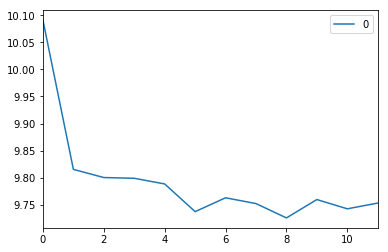
\includegraphics[width=\linewidth]{loss_function.png}
  \caption{A boat.}
  \label{fig:boat1}
\end{figure}

\section{Propostas para melhorar o Baseline.}
A principio, cogitamos utilizar as seguintes estratégias para melhorar o baseline:

\begin{enumerate}

\item Utilização do \textit{Random  Forest}. Esse modelo consiste em
um método  de aprendizado  conjunto para  classificação, regressão
e  outras  tarefas,  que  operam  construindo  uma  multiplicidade  de
árvores  de   decisão  no  momento   do  treinamento  e   gerando  a
classe   que   é   o   modo   das   classes   ou   previsão   média
das   árvores   individuais.   Essa   proposta   foi   discutida   em
\url{https://github.com/henriquepgomide/caRtola/issues/33},  por  esse
motivo resolvemos testá-la para avaliar os resultados.

\item  Acreditamos   também  que   podemos  melhorar   os  resultados
modificando a rede para receber como  entrada não só apenas os dados
de uma terminada rodada, mas sim um histórico das últimas \textit{n}
rodadas.  Isso deve-se  ao fato  de  que, pela  experiencia que  temos
assistindo futebol, o desempenho dos jogadores oscila de acordo com um
determinado histórico. Faremos essa modificação na esperança que o
modelo reconheça esse padrão.

\end{enumerate}

\begin{thebibliography}{00}

\bibitem{git_cartola}      GitHub     -      Repositório     caRtola.
\url{https://github.com/henriquepgomide/caRtola/}.

\bibitem{scikit-learn}  scikit-learn:  machine  learning in  Python  -
\url{http://scikit-learn.org/}, Acessado em 18-10-2018.

\end{thebibliography}

\end{document}
